\documentclass[12pt,a4paper]{article}
\usepackage[utf8]{inputenc}
\usepackage{amsmath}
\usepackage{listings}
\usepackage{verbatim}
\usepackage{graphicx} 
\oddsidemargin 0cm
\marginparwidth 0cm
\hoffset 0cm
\usepackage{polski}
\begin{document} 
\large
\begin{tabular}{|c|c|c|c|}
\hline
\multicolumn{4}{|l|}{Temat:}\\
\multicolumn{4}{|c|}{Rozwiązywanie UARL metodami bezpośrednimi (2)}\\
\hline
\multicolumn{1}{|l}{Wykonał:}&\multicolumn{1}{|l}{Wydział:}&\multicolumn{1}{|c}{Kierunek}&\multicolumn{1}{|l|}{Grupa:}\\
Marcin Fabrykowski&FiIS&Inf. Stos.&grupa 3\\
\hline
\end{tabular}
\normalsize
\vspace{2cm}
\begin{enumerate}
\item Metoda LU\\
Mając równanie Ax=b,\\
gdzie:
\begin{equation}
A=\begin{bmatrix}
a_{11}&a_{12}&a_{13}\\
a_{21}&a_{22}&a_{23}\\
a_{31}&a_{32}&a_{33}
\end{bmatrix}\\
\end{equation}
możemy zapisać powyższe jako iloczyn dwóch macierzy: $A=L*U$, przy czym macierze $L$ i $U$ mają postać:
\begin{equation}
L=
\begin{bmatrix}
1&0&0\\
l_{21}&1&0\\
l_{31}&l_{32}&1
\end{bmatrix}
\end{equation}\\
\begin{equation}
U=
\begin{bmatrix}
u_{11}&u_{12}&u_{13}\\
0&u_{22}&u_{23}\\
0&0&u_{33}
\end{bmatrix}
\end{equation}\\
Wytępuje tutaj zależność:
\begin{equation}
det(A)=det(L\cdot U)=det(L)\cdot det(U)
\end{equation}
następnie wyliczamy kolejno, pierwszy wiersz macierzy $U$, pierwszą kolumnę macierzy $L$, drugi wiersz macierzy $U$, drugą kolumnę macierzy $L$\\
\begin{equation}
\begin{bmatrix}
a_{11}&a_{12}&a_{13}\\
a_{21}&a_{22}&a_{23}\\
a_{31}&a_{32}&a_{33}
\end{bmatrix}=
\begin{bmatrix}
1&0&0\\
l_{21}&1&0\\
l_{31}&l_{32}&1
\end{bmatrix}
\begin{bmatrix}
u_{11}&u_{12}&u_{13}\\
0&u_{22}&u_{23}\\
0&0&u_{33}
\end{bmatrix}
\end{equation}
pierwszy wiersz macierzy $U$:
\begin{align}
\nonumber a_{11}&=1\cdot u_{11}+0\cdot 0+0\cdot 0\\
\nonumber a_{12}&=1\cdot u_{12}+0\cdot u_{22}+0\cdot 0\\
\nonumber a_{13}&=1\cdot u_{13}+0\cdot u_{23}+0\cdot u_{33}
\end{align}
pierwsza kolumna macierzy $L$:
\begin{align}
\nonumber a_{21}&=l_{21}\cdot u_{11}+1\cdot 0+ 0\cdot 0\\
\nonumber a_{31}&=l_{31}\cdot u_{11}+l_{32}\cdot 0+l_{33}\cdot 0
\end{align}
Powyższa procedure powtarzamy dla wszystkich elementów macierzy.
\item Wykonanie ćwiczenia\\
Mając macierz:
\begin{equation}
A=\begin{bmatrix}
2q\cdot 10^{-4}&1&6&9&10\\
2\cdot 10^{-4}&1&6&9&10\\
1&6&6&8&6\\
5&9&10&7&10\\
3&4&9&7&9&
\end{bmatrix}\\
\end{equation}
wyznaczyć zależność wyznacznika $det(A)$ od parametru $q$.\\
W tym celu dokonujemy dekompozycji macierzy $A$ na macierze $L$ i $U$. Używając biblioteki \textit{nrutil}, wykorzystujemy funkcję \textit{ludcmp}. Następnie mając macierze $L$ i $U$, wyliczamamy ich wyznaczniki wykorzystujac właśności macierzy trójkątnych - mnożymy wartości na diagonalach. Następnie mnożymy tak wyliczony wyznaczniki $L$ i $U$ i otrzymujemy wyznacznik macierzy $A$.\\
Oczekiwaną zależność od parametru $a$ przedstawia rys. \ref{fig:plot}
\begin{figure}
\caption{Plot1}
\label{fig:plot}
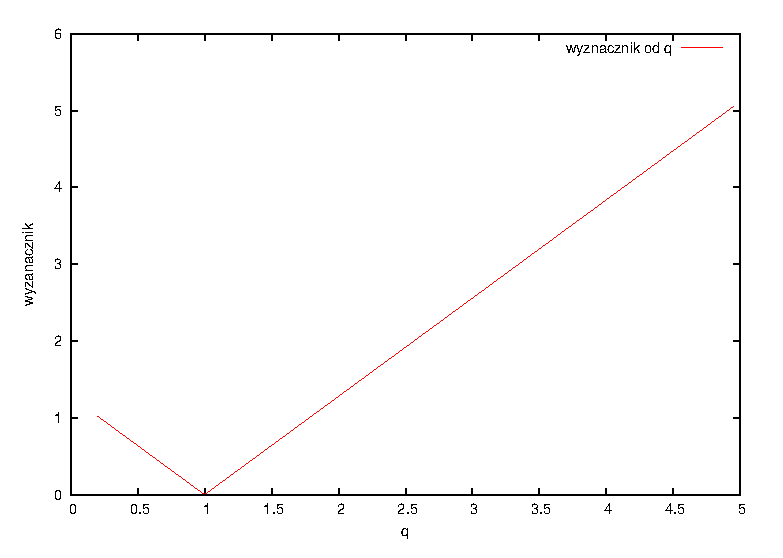
\includegraphics{plot.eps}
\end{figure}
\item Wnioski\\
Metoda LU pozwala w prosty sposób obliczyć wyznacznik macierzy. Proces dekompozycji wymaga wykonania mniejszej ilości operacji, niż wyliczanie wyznacznika innymi metodami co pokazuję zasadność używania tej metody
\end{enumerate}
\end{document}